\documentclass{article}

\usepackage{enumitem}
\usepackage{amsmath}
\usepackage{amsfonts}
\usepackage{amssymb}
\usepackage{textcomp}
\usepackage{tikz}
\usepackage{gensymb}
\usepackage[margin=0.5in]{geometry}
\usepackage[hidelinks]{hyperref}

\makeatletter
\def\input@path{{.}{./img/}}
\makeatother

\let\oldemptyset\emptyset
\let\emptyset\varnothing
\let\oldepsilon\epsilon
\let\epsilon\varepsilon
\newcommand{\N}{\mathbb{N}}

\usepackage{environ}
\NewEnviron{centerframebox}{\begin{center}\fbox{\parbox{0.92\textwidth}{\BODY}}\end{center}}

\title{Combinatorial Optimization \\ Exercise Set 4 \\ Tuesday class}
\author{
  AAAAAAAAAA AAAAAAA \\
  \href{mailto:AAAAAAAAAAAAAAAAAAAA}{AAAAAAAAAAAAAAAAAAAA}
  \and
  Carola Ley \\
  \href{mailto:s6caleyy@uni-bonn.de}{s6caleyy@uni-bonn.de}
  \and
  Bailee Zacovic \\
  \href{mailto:s38bzaco@uni-bonn.de}{s38bzaco@uni-bonn.de}
}

\begin{document}
  \maketitle

  \setcounter{section}{4}
  \subsection{Maximum matching in the graph}
  \begin{centerframebox}
    Find a maximum matching in the graph in Figure 4.1. Prove that
    the matching is indeed maximum, e.g. using the Berge-Tutte-formula.
  \end{centerframebox}
  Consider the matching $M=\{\{1,11\},\{2,7\},\{3,10\},\{4,15\},\{8,13\},\{9,12\},\{14,16\}\},$ where $|M|=7.$ By the Berge-Tutte formula, we recall that $$|V(G)|=2\nu(G)+\underset{X\subset V(G)}{\text{max}}(q_G(X)-|X|).$$Observe that for $X=\{1,8,16\},$ $q_G(X)=5,$ given by the odd connected components $\{5\},\{2,6,7\},\{13\},\{3,9,10,12,14\},$ and $\{11\}.$ It follows that $$\underset{X\subset V(G)}{\text{max}}(q_G(X)-|X|)\geq q_G(\{1,8,16\})-|\{1,8,16\}|=5-3=2.$$ Noting that $|V(G)|=16,$ we obtain
  $$2\nu(G)=16-\underset{X\subset V(G)}{\text{max}}(q_G(X)-|X|)\leq 16-2=14\implies \nu(G)\leq 7.$$ Since $|M|=7,$ it follows that $\nu(G)=7,$ and hence $M$ is indeed maximal. $\blacksquare$

  \subsection{Non-bipartite matching algorithm}
  \begin{centerframebox}
    Recall Exercise 3.2. Although you only had to solve parts (vi)
    and (vii) for bipartite graphs, they can also be solved in general for undirected
    graphs (with the same runtime), only with a more complicated algorithm in part
    (vi). Using this, describe a linear-time approximation scheme for the \textsc{Maximum
    Cardinality Matching Problem}. More specifically, describe an algorithm
    which takes as input an undirected graph $G$ and a positive number $\epsilon$, outputs a
    matching $M$ in $G$ such that $|M| \geq (1 - \epsilon) \cdot \nu(G)$, and runs in

    $$ O\left(\frac{1}{\epsilon} \cdot (|V (G)| + |E(G)|) \right)\textrm{-time.} $$
  \end{centerframebox}
  First, let's assume, without loss of generality, that the factor $\epsilon$ is in the form $\epsilon = \frac{1}{\kappa}$, where $\kappa \in \N$.
  This doesn't matter for the time complexity, because it's inside the big $O()$ asymptotic function,
  and it also doesn't matter for the inequality $|M| \geq (1 - \epsilon) \cdot \nu(G)$, because we can round down, and still satisfy it.

  Recall how in Exercise 3.2 part (v) we considered how the sequence of augmenting path lengths has a lot of repeating numbers,
  and our algorithm took $O(|V (G)| + |E(G)|)$ time to process such a group of consecutive same length augmenting paths.
  We looked at the unique odd values of $\frac{\nu(G)+|M|}{\nu(G)-|M|}$, reframed as $f(x) = \left\lfloor\frac{\nu(G)}{x}\right\rfloor$, where $x$ goes down from $\nu(G)$ to $0$.
  In our case it will be useful to think of $x$ as the number of matching edges we still need to get for a maximum matching, and for our approximation we only need to consider the values of $x \geq \epsilon\nu(G)$.

  If $\kappa \geq \sqrt{\nu(G)}$, then we can get away with just running the full algorithm, because its $O(\sqrt{n}(n+m))$ time complexity, will be better then our desired $O(\kappa \cdot (n+m))$.
  This way we only have to consider the cases where $\kappa < \sqrt{\nu(G)}$.
  Then we look at out function $f(x)$ and when it equals a particular value $\kappa$ and solve for $x$.
  Because we have already established $\kappa < \sqrt{\nu(G)}$, all values of this function will repeat at least once,
  and we don't have to worry about some of them getting missed because of the rounding.
  \[ \frac{\nu(G)}{x'} = \kappa \]
  \[ x' = \frac{\nu(G)}{\kappa} \]
  So $x'$ becomes a particular value of $x$ at which the function $f(x)$ starts to return values $\geq \kappa$,
  and for all $\forall x \geq x' : f(x) \leq \kappa$.
  This way the number of unique values $f(x > x')$ can produce is exactly $\kappa$,
  as every value must appear at least once and the lowest possible one is $1$.
  The amount of unique inputs $f(x > x')$ can take is just $\max x - x' = \nu(G) - x'$.
  %  = \nu(G) - \frac{\nu(G)}{\kappa}

  This means that if we program our approximation algorithm to only take the first $\kappa$ steps,
  it would have added $\nu(G) - x'$ matching edges, one for each input value $x$ to our function $f(x)$.
  Considering the approximation inequality again:
  \begin{align*}
    |M| &\geq (1 - \epsilon) \cdot \nu(G) \\
    |M| &\geq (1 - \frac{1}{\kappa}) \cdot \nu(G) \\
    |M| &\geq \nu(G) - \frac{\nu(G)}{\kappa} \\
    |M| &\geq \nu(G) - x'
  \end{align*}
  And we have already established that we have $\nu(G) - x'$ matching edges.
  We can see that our new approximation algorithm satisfies the inequality and its runtime is $O(\kappa \cdot (n+m))$, as requested.
  $\blacksquare$

  \subsection{3-regular undirected graph}
  \begin{centerframebox}
    Let G be a 3-regular undirected graph.
    \begin{enumerate}[label=(\alph*)]
      \item Assume $G$ is simple. Show that there is a matching in $G$ covering at least
      $(7/8) \cdot |V (G)|$ vertices.
      \item Give an example to prove that the bound of item (a) is tight.
      \item Show that the assumption that $G$ is simple in item (a) is necessary.
    \end{enumerate}
  \end{centerframebox}
  (a) Let $G$ be a simple, $3$-regular graph. We first note that $$2\cdot |E(G)|=\sum_{v\in V(G)}\text{deg}(v)=3\cdot |V(G)|,$$hence $|V(G)|$ is even. By the Berge-Tutte formula, it suffices to show $q_G(X)-|X|\leq \frac{|V(G)|}{8}$ for all $X\subset V(G).$ To this end, fix $X\subset V(G).$ Since $G$ is $3$-regular, any connected components of $G$ \textit{not} containing vertices in $X$ are even by previous argument, and thus will not be counted by $q_G(X).$

  Thus, it suffices to consider those odd components $C_i$ of $G-X$ where at least one edge joins a vertex in $C_i$ to a vertex in $X.$ When $|V(C_i)|=1$ or $3$, there must be exactly three edges joining vertices in $C_i$ to vertices in $X$, since $G$ is $3$-regular and simple. When $|V(C_i)|\geq 5,$ there is at least one such edge.
  Let $m$ denote the number of $C_i$ containing exactly $1$ or $3$ vertices; let $n$ denote the number of $C_i$ containing $5$ or more vertices. Then $q_G(X)=n+m.$ It follows that
  \begin{align*}
      3\cdot |X|=|\{\text{edges leaving }X\}|=|\{\text{edges entering }C_i\text{ for all }i\}|\geq 3m+n
  \end{align*}
  and
  \begin{align*}
      |V(G)|-|X|\geq n+5m.
  \end{align*}
  Combining these two bounds, we discover
  $$8\cdot(q_G(X)-|X|)\leq 8\cdot (n+m)-8\cdot \left(m+\frac{n}{3}\right)=\frac{16n}{3}\leq 2m+\frac{16n}{3}=\left(m+\frac{n}{3}\right)+(m+5n)\leq |X|+(|V(G)|-|X|)=|V(G)|.$$In short,
  $$q_G(X)-|X|\leq \frac{|V(G)|}{8}.$$ Since $X\subset V(G)$ was arbitrary, it follows by the Berge-Tutte formula that,

  $$2\nu(G)=|V(G)|-\underset{X\subset V(G)}{\text{max}}(q_G(X)-|X|)\geq |V(G)|-\frac{|V(G)|}{8}=\frac{7}{8}|V(G)|.$$
  In other words, there exists a maximum matching of $G$ covering $2\nu(G)\geq \frac{7}{8}|V(G)|$ vertices. $\blacksquare$




  \newpage
  %It follows that $q_G(X)\leq 3\cdot |X|$ (since each vertex in $X$ induces at most $3$ odd connected components), and hence $q_G(X)-|X|\leq 2\cdot |X|.$ On the other hand,

  (b) Consider the following simple graph $G$:

  \begin{figure}[h]
  \begin{center}
    \tikzset{
    unmarked/.style args={}{
        draw, fill=black, circle, inner sep=0pt, minimum size=.25cm,
    }
}

\tikzset{
    marked/.style args={}{
        draw, fill=white, circle, inner sep=0pt, minimum size=0.25cm, line width=0.06cm
    }
}



\tikzset{every picture/.style={line width=0.75pt}} %set default line width to 0.75pt

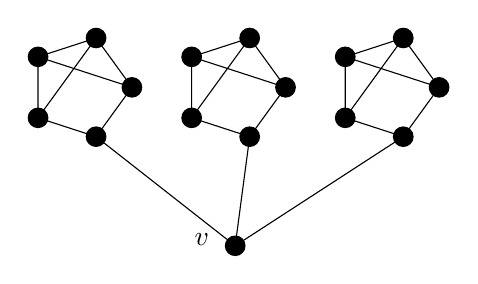
\begin{tikzpicture}[x=0.75pt,y=0.75pt,yscale=-1,xscale=1]
%uncomment if require: \path (0,300); %set diagram left start at 0, and has height of 300

%Shape: Ellipse [id:dp6157615359367345]
\draw  [fill={rgb, 255:red, 0; green, 0; blue, 0 }  ,fill opacity=1 ] (277.73,196.65) .. controls (280.34,196.64) and (282.46,198.73) .. (282.47,201.31) .. controls (282.49,203.9) and (280.39,206.01) .. (277.78,206.03) .. controls (275.17,206.04) and (273.05,203.96) .. (273.03,201.37) .. controls (273.02,198.78) and (275.12,196.67) .. (277.73,196.65) -- cycle ;
%Shape: Ellipse [id:dp6097862782932393]
\draw  [fill={rgb, 255:red, 0; green, 0; blue, 0 }  ,fill opacity=1 ] (284.7,96.54) .. controls (287.31,96.52) and (289.43,98.61) .. (289.45,101.2) .. controls (289.46,103.78) and (287.36,105.9) .. (284.75,105.91) .. controls (282.14,105.93) and (280.02,103.84) .. (280,101.25) .. controls (279.99,98.66) and (282.09,96.55) .. (284.7,96.54) -- cycle ;
%Shape: Ellipse [id:dp23517382164865208]
\draw  [fill={rgb, 255:red, 0; green, 0; blue, 0 }  ,fill opacity=1 ] (256.75,105.62) .. controls (259.36,105.6) and (261.48,107.69) .. (261.5,110.28) .. controls (261.51,112.87) and (259.41,114.98) .. (256.8,114.99) .. controls (254.19,115.01) and (252.07,112.92) .. (252.05,110.33) .. controls (252.04,107.74) and (254.14,105.63) .. (256.75,105.62) -- cycle ;
%Shape: Ellipse [id:dp386601276783894]
\draw  [fill={rgb, 255:red, 0; green, 0; blue, 0 }  ,fill opacity=1 ] (256.75,135.01) .. controls (259.36,134.99) and (261.48,137.08) .. (261.5,139.67) .. controls (261.51,142.26) and (259.41,144.37) .. (256.8,144.38) .. controls (254.19,144.4) and (252.07,142.31) .. (252.05,139.72) .. controls (252.04,137.13) and (254.14,135.02) .. (256.75,135.01) -- cycle ;
%Shape: Ellipse [id:dp3904586665893117]
\draw  [fill={rgb, 255:red, 0; green, 0; blue, 0 }  ,fill opacity=1 ] (301.97,120.31) .. controls (304.58,120.3) and (306.71,122.38) .. (306.72,124.97) .. controls (306.73,127.56) and (304.63,129.67) .. (302.03,129.69) .. controls (299.42,129.7) and (297.29,127.62) .. (297.28,125.03) .. controls (297.27,122.44) and (299.37,120.33) .. (301.97,120.31) -- cycle ;
%Shape: Ellipse [id:dp07425790402378452]
\draw  [fill={rgb, 255:red, 0; green, 0; blue, 0 }  ,fill opacity=1 ] (284.7,144.09) .. controls (287.31,144.07) and (289.43,146.16) .. (289.45,148.75) .. controls (289.46,151.34) and (287.36,153.45) .. (284.75,153.46) .. controls (282.14,153.48) and (280.02,151.39) .. (280,148.8) .. controls (279.99,146.22) and (282.09,144.1) .. (284.7,144.09) -- cycle ;
%Shape: Regular Polygon [id:dp9690298828443213]
\draw   (302,125) -- (284.73,148.78) -- (256.77,139.69) -- (256.77,110.31) -- (284.73,101.22) -- cycle ;
%Shape: Ellipse [id:dp42574462708286176]
\draw  [fill={rgb, 255:red, 0; green, 0; blue, 0 }  ,fill opacity=1 ] (330.75,105.62) .. controls (333.36,105.6) and (335.48,107.69) .. (335.5,110.28) .. controls (335.51,112.87) and (333.41,114.98) .. (330.8,114.99) .. controls (328.19,115.01) and (326.07,112.92) .. (326.05,110.33) .. controls (326.04,107.74) and (328.14,105.63) .. (330.75,105.62) -- cycle ;
%Shape: Ellipse [id:dp11996344977034723]
\draw  [fill={rgb, 255:red, 0; green, 0; blue, 0 }  ,fill opacity=1 ] (330.75,135.01) .. controls (333.36,134.99) and (335.48,137.08) .. (335.5,139.67) .. controls (335.51,142.26) and (333.41,144.37) .. (330.8,144.38) .. controls (328.19,144.4) and (326.07,142.31) .. (326.05,139.72) .. controls (326.04,137.13) and (328.14,135.02) .. (330.75,135.01) -- cycle ;
%Shape: Ellipse [id:dp11091416244121066]
\draw  [fill={rgb, 255:red, 0; green, 0; blue, 0 }  ,fill opacity=1 ] (375.97,120.31) .. controls (378.58,120.3) and (380.71,122.38) .. (380.72,124.97) .. controls (380.73,127.56) and (378.63,129.67) .. (376.03,129.69) .. controls (373.42,129.7) and (371.29,127.62) .. (371.28,125.03) .. controls (371.27,122.44) and (373.37,120.33) .. (375.97,120.31) -- cycle ;
%Shape: Ellipse [id:dp28940132669054863]
\draw  [fill={rgb, 255:red, 0; green, 0; blue, 0 }  ,fill opacity=1 ] (358.7,144.09) .. controls (361.31,144.07) and (363.43,146.16) .. (363.45,148.75) .. controls (363.46,151.34) and (361.36,153.45) .. (358.75,153.46) .. controls (356.14,153.48) and (354.02,151.39) .. (354,148.8) .. controls (353.99,146.22) and (356.09,144.1) .. (358.7,144.09) -- cycle ;
%Shape: Regular Polygon [id:dp797135067353866]
\draw   (376,125) -- (358.73,148.78) -- (330.77,139.69) -- (330.77,110.31) -- (358.73,101.22) -- cycle ;
%Shape: Ellipse [id:dp6565560372458352]
\draw  [fill={rgb, 255:red, 0; green, 0; blue, 0 }  ,fill opacity=1 ] (210.7,96.54) .. controls (213.31,96.52) and (215.43,98.61) .. (215.45,101.2) .. controls (215.46,103.78) and (213.36,105.9) .. (210.75,105.91) .. controls (208.14,105.93) and (206.02,103.84) .. (206,101.25) .. controls (205.99,98.66) and (208.09,96.55) .. (210.7,96.54) -- cycle ;
%Shape: Ellipse [id:dp9125644190023552]
\draw  [fill={rgb, 255:red, 0; green, 0; blue, 0 }  ,fill opacity=1 ] (182.75,105.62) .. controls (185.36,105.6) and (187.48,107.69) .. (187.5,110.28) .. controls (187.51,112.87) and (185.41,114.98) .. (182.8,114.99) .. controls (180.19,115.01) and (178.07,112.92) .. (178.05,110.33) .. controls (178.04,107.74) and (180.14,105.63) .. (182.75,105.62) -- cycle ;
%Shape: Ellipse [id:dp08349267618583034]
\draw  [fill={rgb, 255:red, 0; green, 0; blue, 0 }  ,fill opacity=1 ] (182.75,135.01) .. controls (185.36,134.99) and (187.48,137.08) .. (187.5,139.67) .. controls (187.51,142.26) and (185.41,144.37) .. (182.8,144.38) .. controls (180.19,144.4) and (178.07,142.31) .. (178.05,139.72) .. controls (178.04,137.13) and (180.14,135.02) .. (182.75,135.01) -- cycle ;
%Shape: Ellipse [id:dp9107142788834091]
\draw  [fill={rgb, 255:red, 0; green, 0; blue, 0 }  ,fill opacity=1 ] (227.97,120.31) .. controls (230.58,120.3) and (232.71,122.38) .. (232.72,124.97) .. controls (232.73,127.56) and (230.63,129.67) .. (228.03,129.69) .. controls (225.42,129.7) and (223.29,127.62) .. (223.28,125.03) .. controls (223.27,122.44) and (225.37,120.33) .. (227.97,120.31) -- cycle ;
%Shape: Ellipse [id:dp2920739309601139]
\draw  [fill={rgb, 255:red, 0; green, 0; blue, 0 }  ,fill opacity=1 ] (210.7,144.09) .. controls (213.31,144.07) and (215.43,146.16) .. (215.45,148.75) .. controls (215.46,151.34) and (213.36,153.45) .. (210.75,153.46) .. controls (208.14,153.48) and (206.02,151.39) .. (206,148.8) .. controls (205.99,146.22) and (208.09,144.1) .. (210.7,144.09) -- cycle ;
%Shape: Regular Polygon [id:dp46188853209567804]
\draw   (228,125) -- (210.73,148.78) -- (182.77,139.69) -- (182.77,110.31) -- (210.73,101.22) -- cycle ;
%Straight Lines [id:da4307039265371213]
\draw    (210.73,148.78) -- (277.75,201.34) ;
%Straight Lines [id:da48834390538516237]
\draw    (358.73,148.78) -- (277.75,201.34) ;
%Straight Lines [id:da09750211059585712]
\draw    (284.73,148.78) -- (277.75,201.34) ;
%Straight Lines [id:da7469775847793634]
\draw    (358.73,101.22) -- (330.77,139.69) ;
%Straight Lines [id:da47531016673102666]
\draw    (376,125) -- (330.77,110.31) ;
%Straight Lines [id:da8201975105389097]
\draw    (284.73,101.22) -- (256.77,139.69) ;
%Straight Lines [id:da49067451893021485]
\draw    (302,125) -- (256.77,110.31) ;
%Straight Lines [id:da8003123870638236]
\draw    (210.73,101.22) -- (182.77,139.69) ;
%Straight Lines [id:da8106168954060751]
\draw    (228,125) -- (182.77,110.31) ;
%Shape: Ellipse [id:dp44152660781155584]
\draw  [fill={rgb, 255:red, 0; green, 0; blue, 0 }  ,fill opacity=1 ] (358.7,96.54) .. controls (361.31,96.52) and (363.43,98.61) .. (363.45,101.2) .. controls (363.46,103.78) and (361.36,105.9) .. (358.75,105.91) .. controls (356.14,105.93) and (354.02,103.84) .. (354,101.25) .. controls (353.99,98.66) and (356.09,96.55) .. (358.7,96.54) -- cycle ;

% Text Node
\draw (257,194.4) node [anchor=north west][inner sep=0.75pt]    {$v$};


\end{tikzpicture}



    \end{center}
  \end{figure}
  Notice that $q_G(\{v\})-|\{v\}|=2,$ and so by Berge-Tutte: $$2\nu(G)=|V(G)|-\underset{X\subset V(G)}{\text{max}}(q_G(X)-|X|)\leq 16-2=14$$which implies that $\nu(G)\leq 7.$ By part (a), there exists a maximum matching covering at least $$14=(7/8)\cdot 16=(7/8)\cdot |V(G)|$$vertices of $G,$ and so it must happen that $\nu(G)=7,$ i.e. the bound demonstrated in (a) is tight at this particular $G$. $\blacksquare$

  (c) Consider the following non-simple graph $G$:

  \begin{figure}[h]
  \begin{center}
    \tikzset{
    unmarked/.style args={}{
        draw, fill=black, circle, inner sep=0pt, minimum size=.25cm,
    }
}

\tikzset{
    marked/.style args={}{
        draw, fill=white, circle, inner sep=0pt, minimum size=0.25cm, line width=0.06cm
    }
}



\tikzset{every picture/.style={line width=0.75pt}} %set default line width to 0.75pt

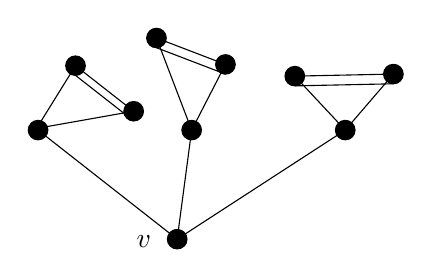
\begin{tikzpicture}[x=0.75pt,y=0.75pt,yscale=-1,xscale=1]
%uncomment if require: \path (0,300); %set diagram left start at 0, and has height of 300

%Shape: Ellipse [id:dp6157615359367345]
\draw  [fill={rgb, 255:red, 0; green, 0; blue, 0 }  ,fill opacity=1 ] (277.73,196.65) .. controls (280.34,196.64) and (282.46,198.73) .. (282.47,201.31) .. controls (282.49,203.9) and (280.39,206.01) .. (277.78,206.03) .. controls (275.17,206.04) and (273.05,203.96) .. (273.03,201.37) .. controls (273.02,198.78) and (275.12,196.67) .. (277.73,196.65) -- cycle ;
%Shape: Ellipse [id:dp386601276783894]
\draw  [fill={rgb, 255:red, 0; green, 0; blue, 0 }  ,fill opacity=1 ] (256.75,135.01) .. controls (259.36,134.99) and (261.48,137.08) .. (261.5,139.67) .. controls (261.51,142.26) and (259.41,144.37) .. (256.8,144.38) .. controls (254.19,144.4) and (252.07,142.31) .. (252.05,139.72) .. controls (252.04,137.13) and (254.14,135.02) .. (256.75,135.01) -- cycle ;
%Shape: Ellipse [id:dp07425790402378452]
\draw  [fill={rgb, 255:red, 0; green, 0; blue, 0 }  ,fill opacity=1 ] (284.7,144.09) .. controls (287.31,144.07) and (289.43,146.16) .. (289.45,148.75) .. controls (289.46,151.34) and (287.36,153.45) .. (284.75,153.46) .. controls (282.14,153.48) and (280.02,151.39) .. (280,148.8) .. controls (279.99,146.22) and (282.09,144.1) .. (284.7,144.09) -- cycle ;
%Shape: Ellipse [id:dp11996344977034723]
\draw  [fill={rgb, 255:red, 0; green, 0; blue, 0 }  ,fill opacity=1 ] (381.89,117.1) .. controls (384.5,117.08) and (386.62,119.17) .. (386.64,121.76) .. controls (386.65,124.35) and (384.55,126.46) .. (381.94,126.47) .. controls (379.33,126.49) and (377.21,124.4) .. (377.19,121.81) .. controls (377.18,119.22) and (379.28,117.11) .. (381.89,117.1) -- cycle ;
%Shape: Ellipse [id:dp28940132669054863]
\draw  [fill={rgb, 255:red, 0; green, 0; blue, 0 }  ,fill opacity=1 ] (358.7,144.09) .. controls (361.31,144.07) and (363.43,146.16) .. (363.45,148.75) .. controls (363.46,151.34) and (361.36,153.45) .. (358.75,153.46) .. controls (356.14,153.48) and (354.02,151.39) .. (354,148.8) .. controls (353.99,146.22) and (356.09,144.1) .. (358.7,144.09) -- cycle ;
%Shape: Ellipse [id:dp08349267618583034]
\draw  [fill={rgb, 255:red, 0; green, 0; blue, 0 }  ,fill opacity=1 ] (334.4,118.09) .. controls (337.01,118.08) and (339.13,120.16) .. (339.15,122.75) .. controls (339.16,125.34) and (337.06,127.45) .. (334.45,127.47) .. controls (331.84,127.48) and (329.72,125.4) .. (329.7,122.81) .. controls (329.69,120.22) and (331.79,118.11) .. (334.4,118.09) -- cycle ;
%Shape: Ellipse [id:dp9107142788834091]
\draw  [fill={rgb, 255:red, 0; green, 0; blue, 0 }  ,fill opacity=1 ] (228.74,113.06) .. controls (231.35,113.04) and (233.47,115.13) .. (233.49,117.72) .. controls (233.5,120.31) and (231.4,122.42) .. (228.79,122.43) .. controls (226.18,122.45) and (224.06,120.36) .. (224.04,117.77) .. controls (224.03,115.18) and (226.13,113.07) .. (228.74,113.06) -- cycle ;
%Shape: Ellipse [id:dp2920739309601139]
\draw  [fill={rgb, 255:red, 0; green, 0; blue, 0 }  ,fill opacity=1 ] (210.7,144.09) .. controls (213.31,144.07) and (215.43,146.16) .. (215.45,148.75) .. controls (215.46,151.34) and (213.36,153.45) .. (210.75,153.46) .. controls (208.14,153.48) and (206.02,151.39) .. (206,148.8) .. controls (205.99,146.22) and (208.09,144.1) .. (210.7,144.09) -- cycle ;
%Straight Lines [id:da4307039265371213]
\draw    (210.73,148.78) -- (277.75,201.34) ;
%Straight Lines [id:da48834390538516237]
\draw    (358.73,148.78) -- (277.75,201.34) ;
%Straight Lines [id:da09750211059585712]
\draw    (284.73,148.78) -- (277.75,201.34) ;
%Shape: Triangle [id:dp13555777212175668]
\draw   (228.76,117.75) -- (256.77,139.69) -- (210,147.98) -- cycle ;
%Shape: Triangle [id:dp0675108284609165]
\draw   (358.73,148.78) -- (334.43,122.78) -- (381.92,121.78) -- cycle ;
%Shape: Triangle [id:dp1406844325804908]
\draw   (301,117.13) -- (284.73,148.78) -- (267.77,104.4) -- cycle ;
%Shape: Ellipse [id:dp1365076686256248]
\draw  [fill={rgb, 255:red, 0; green, 0; blue, 0 }  ,fill opacity=1 ] (300.98,112.45) .. controls (303.59,112.43) and (305.71,114.52) .. (305.72,117.11) .. controls (305.74,119.69) and (303.64,121.8) .. (301.03,121.82) .. controls (298.42,121.83) and (296.3,119.75) .. (296.28,117.16) .. controls (296.27,114.57) and (298.37,112.46) .. (300.98,112.45) -- cycle ;
%Shape: Ellipse [id:dp24236222529832818]
\draw  [fill={rgb, 255:red, 0; green, 0; blue, 0 }  ,fill opacity=1 ] (267.75,99.72) .. controls (270.35,99.7) and (272.48,101.79) .. (272.49,104.38) .. controls (272.51,106.97) and (270.41,109.08) .. (267.8,109.09) .. controls (265.19,109.11) and (263.07,107.02) .. (263.05,104.43) .. controls (263.04,101.84) and (265.14,99.73) .. (267.75,99.72) -- cycle ;
%Straight Lines [id:da0057455971898583424]
\draw    (228.79,122.43) -- (256.8,144.38) ;
%Straight Lines [id:da5660132727377674]
\draw    (267.8,109.09) -- (301.03,121.82) ;
%Straight Lines [id:da17117560906894091]
\draw    (334.45,127.47) -- (381.94,126.47) ;

% Text Node
\draw (257,198.4) node [anchor=north west][inner sep=0.75pt]    {$v$};


\end{tikzpicture}

    \end{center}
  \end{figure}

  As in part (b), notice that $q_G(\{v\})-|\{v\}|=2,$ and so by Berge-Tutte: $$2\nu(G)=|V(G)|-\underset{X\subset V(G)}{\text{max}}(q_G(X)-|X|)\leq 10-2=8$$which implies that $\nu(G)\leq 4,$ i.e. any maximum matching covers at most $8$ vertices. However, the result from part (a) would guarantee a matching covering at least $ (7/8)\cdot 10>8$ vertices. Hence the assumption that $G$ is simple in (a) is necessary. $\blacksquare$

  \subsection{Gallai-Edmonds decompositions}
  \begin{centerframebox}
    Let $G$ be any graph and denote by $Y,\, X,\, W$ its Gallai-Edmonds decomposition.
    Let $v \in X$ and denote by $Y',\, X',\, W'$ the Gallai-Edmonds decomposition of $G - v$.
    Show that $Y' = Y,\, X' = X \setminus \{v\},\, W' = W$.
  \end{centerframebox}
  As $v\in X$ it is covered by every maximum matching in $G$, removing this edge leads to a matching in $G-v$. If there was a larger matching in $G-v$ it would be a maximum matching in $G$ exposing $v$ which is a contradiction to $v\in X$. Thus $\nu(G)=\nu(G-v)+1$.

  For every $y\in Y$ there is a maximum matching $M$ in $G$ exposing $y$. Let $w$ be the vertex with $\{v,w\}\in M$, by Theorem 1.52 $w\in Y$. $M\setminus \{\{v,w\}\}$ is a matching in $G-v$  of size $\nu(G)-1$, thus a maximum matching exposing $y$. As there is such a maximum  matching in $G-v$ for every $y\in Y$ it is $Y\subseteq Y'$.

  Suppose there is a vertex $a\in Y'\setminus Y$, then there is a maximum matching $M'$ in $G-v$ exposing $a$. If $a$ was a neighbour of $v$, then there is a maximum matching in $G$ containing $\{a,v\}$, so by Theorem 1.52 $a\in Y$ which is a contradiction, thus $\{a,v\}\notin E(G)$. As $|M'|=\nu(G)-1$, $a\notin Y$ and $v\in X$ there is an shortest $M'$-augmenting path $P$ in $G$ going from $a$ to $v$. %If $a\in W$ there is a maximum matching in $G$ with an edge from $X$ to $W$ which is a contradiction to Theorem 1.52. As $a\notin Y\cup W$ it is $a\in X$.
  $P$ can only use edges between $X$ and $Y$ and within $Y$, as otherwise the resulting maximum matching in $G$ contains an edge within $X$ or between $X$ and $W$ which is a contradiction to Theorem 1.52. As $a$ is no neighbour of $v$, $P$ must contain at least one vertex of $Y$. As all connected components of $G[Y]$ are factor-critical, $P$ has an even number of edges within each connected component of $G[Y]$ and thus even length from one vertex in $X$ to an other vertex in $X$. As every augmenting path has odd length, it must contain an edge within $X$ which is a contradiction to Theorem 1.52. Thus there is no $M'$-augmenting path in $G$ between $a$ and $v$, which is a contradiction to $M'$ being a matching of size $\nu(G)-1$. Therefore there is no vertex in $Y'\setminus Y$, so $Y=Y'$.

  From $Y=Y'$ it follows that $X=\Gamma_{G}(Y)=\Gamma_{G-v}(Y)\cup \{v\}=X' \cup \{v\} \Rightarrow X' = X \setminus \{v\}$ and $W=V(G)\setminus (Y\cup X)=V(G)\setminus (Y'\cup X'\cup \{v\})=W'$.
\end{document}

